% ThaiEditBench --- ACL paper, camera-ready.  COMPILE WITH LuaLaTeX (not pdfLaTeX): Thai
% script needs fontspec + babel font-switching.  On Overleaf set the compiler to LuaLaTeX.
% Build:  lualatex -> bibtex -> lualatex -> lualatex   (or latexmk -lualatex)
\documentclass[11pt]{article}

\usepackage[final]{acl}

\usepackage{microtype}
\usepackage{graphicx}
\usepackage{booktabs}
\usepackage{amssymb}
\usepackage{amsmath}

% Let a wide (two-column) table occupy more of a page top.
\renewcommand{\dbltopfraction}{0.92}
\renewcommand{\dblfloatpagefraction}{0.8}
\renewcommand{\topfraction}{0.9}
\renewcommand{\textfraction}{0.07}

% --- Fonts / scripts (LuaLaTeX or XeLaTeX only) -----------------------------
\usepackage[english]{babel}
\babelfont{rm}{TeX Gyre Termes}            % Times-like for Latin
% Auto-switch to a Thai font whenever Thai-script characters appear, so inline
% Thai needs no wrapping.  The Thai font is BUNDLED in fonts/ (Noto Serif Thai).
\babelprovide[import, onchar=ids fonts]{thai}
\babelfont[thai]{rm}[Path=fonts/, Extension=.ttf,
  UprightFont=NotoSerifThai-Regular, BoldFont=NotoSerifThai-Bold]{NotoSerifThai}
% ----------------------------------------------------------------------------

% Statistically tied with the column best (paired item bootstrap, p >= 0.05).
\newcommand{\tie}[1]{\underline{#1}}

\title{ThaiEditBench: A Mechanism-Typed, Length-Stratified Benchmark\\
       for Thai Orthographic Error Correction}

\author{Nutchanon Yongsatianchot\textsuperscript{1} \quad
        Piyalitt Ittichaiwong\textsuperscript{2} \quad
        Kanyakorn Veerakanjana\textsuperscript{2} \\
        \textsuperscript{1}Siriraj Genomics \quad
        \textsuperscript{2}Siriraj Informatics and Data Innovation Center (SIData+) \\
        Faculty of Medicine Siriraj Hospital, Mahidol University}

\begin{document}
\maketitle

\begin{abstract}
Thai is written without word boundaries and layers tone marks, silent consonants, and heavy
loanword transliteration onto a Brahmic script. This produces orthographic error mechanisms
unlike those targeted by English grammatical error correction (GEC) or Chinese spelling check
(CSC). We present \textbf{ThaiEditBench}, a character-level Thai orthographic error-correction
benchmark with three components: (i) a \textbf{six-class mechanism taxonomy} plus an etymology
tag; (ii) \textbf{three length tiers} (sentence, paragraph, and page) that isolate robustness to
long, mostly-clean context; and (iii) \textbf{contamination-robust construction}, in which
naturally attested misspellings are \emph{injected} into novel clean text screened by a
memorization probe. Gold corrections are exact by construction, and a blind two-annotator study
shows that the taxonomy can be applied reliably (Krippendorff's $\alpha = 0.75$). Grading is at
the character-cluster level with span-based matching adapted from ERRANT. Evaluating
\textbf{16 models}, we find that (1) under the benchmark's conditions, models that locate an
error almost always fix it correctly, so what separates them is \emph{detection}; (2) the
evaluated Thai-specialized models do not lead the strongest general models; and (3) long,
mostly-correct context exposes \textbf{over-edit accumulation} and clean-text fidelity failures
that sentence-level evaluation hides. On real errors mined from Wikipedia edit history, scores
are somewhat lower but the model ranking transfers (Spearman $\rho = 0.92$).
\end{abstract}

\section{Introduction}

Thai orthography is error-prone in script-specific ways: tone-mark selection and placement,
silent-consonant marks, homophonous consonants, vowel-form confusions, consonant-cluster
metathesis, and inconsistent loanword transliteration. These are \textbf{character-level}
errors that turn on \textbf{specific mechanisms}, and Thai's lack of whitespace word
boundaries makes them hard to localize and score with token-based tools. Yet the resources to
study them are missing. Grammatical-error-correction benchmarks are English-centric
\citep{bryant-etal-2017-automatic,bryant-etal-2019-bea,napoles-etal-2017-jfleg}, and the
closest character-level analogue is Chinese spelling check
\citep{tseng-etal-2015-introduction,liu-etal-2011-visually}. For Thai, existing
error-annotated resources are social-media, informal, or learner-domain
\citep{lertpiya-etal-2020-thai,nakwijit-purver-2022-misspelling}, and there is no
formal-register, mechanism-typed, contamination-controlled orthographic benchmark.
Document-level and context-aware GEC study correction over long context
\citep{yuan-bryant-2021-document}, but no benchmark isolates length and error-sparsity
robustness for Thai orthographic correction.

\noindent\textbf{Contributions.}
(1)~\textbf{ThaiEditBench}, a character-level Thai orthographic correction benchmark with a
six-class mechanism taxonomy plus an etymology tag and \textbf{three length tiers} (sentence,
paragraph, page). It is \textbf{contamination-robust by construction}: naturally attested
misspellings are injected into novel clean text screened by a memorization probe, so gold
corrections are exact. A blind annotation study measures how reliably the taxonomy can be applied
(Krippendorff's $\alpha = 0.75$).
(2)~An \textbf{ERRANT-style orthographic edit-typer for Thai} that aligns edits at TCC level
and labels each with one of the six mechanism classes, enabling \textbf{per-mechanism
span-F0.5} (cf.\ ChERRANT's dual-granularity scoring \citep{zhang-etal-2022-mucgec}). We use it
as a scoring and diagnosis instrument, not as a general Thai grammatical error classifier.
(3)~A \textbf{16-model evaluation}: models that find an error almost always fix it, so detection
separates them; the evaluated Thai-specialized systems do not lead; weaker models accumulate
over-edits under long context; and the ranking transfers to naturally occurring errors
(Spearman $\rho = 0.92$).
We release code, data, grader, edit-typer, and the variant map at
\url{https://github.com/yongsa-nut/ThaiEditBench}.

\section{Related Work}

\noindent\textbf{GEC and CSC.} English grammatical error correction is evaluated with
span-based metrics. The M\textsuperscript{2} scorer matches a system's edits against gold edit
spans \citep{dahlmeier-ng-2012-better}, ERRANT (the ERRor ANnotation Toolkit) additionally
infers an error type for each edit automatically and reports an F0.5 score
\citep{bryant-etal-2017-automatic}, and GLEU measures
fluency \citep{napoles-etal-2015-ground}. ERRANT-style span matching aligns the wrong and
corrected text into a minimal set of edit spans, then credits a system for each gold span it
recovers with the correct replacement; we adapt this scheme to Thai TCC units
(Section~\ref{sec:typer}). Character-level Chinese spelling check is the closest task, scoring
position-based detection and correction F1 without word boundaries
\citep{tseng-etal-2015-introduction,wu-etal-2013-chinese,yu-etal-2014-overview}, with
confusion-set construction \citep{liu-etal-2011-visually} and the MuCGEC/ChERRANT
dual-granularity scorer \citep{zhang-etal-2022-mucgec}. ERRANT has been ported to Arabic
\citep{belkebir-habash-2021-automatic} and Korean \citep{yoon-etal-2023-towards}, but not Thai.
Wikipedia-revision mining of typo pairs is established for English
\citep{grundkiewicz-junczysdowmunt-2014-wiked} and Japanese
\citep{tanaka-etal-2020-building}.

\noindent\textbf{Thai NLP.} We build on PyThaiNLP for tokenization and dictionary tooling
\citep{phatthiyaphaibun-etal-2023-pythainlp} and on the Thai Character Cluster as the minimal
orthographic unit \citep{theeramunkong-etal-2000-character}. Prior Thai spelling correction
targets social text \citep{lertpiya-etal-2020-thai,lertpiya-etal-2023-progressively}, and
related work studies the semantics of Thai misspellings
\citep{nakwijit-purver-2022-misspelling}. The VISTEC-TP-TH-2021 Twitter corpus includes
misspelling detection and correction as well as word-segmentation annotation, but it is
informal Twitter text rather than a formal-register, mechanism-typed orthographic benchmark
\citep{limkonchotiwat-etal-2021-handling}.

\section{The ThaiEditBench Benchmark}

\subsection{Task}
Given a Thai passage containing character-level orthographic errors, return the passage with
those errors corrected and \textbf{nothing else changed}: no rewriting, re-spacing, numeral,
or punctuation edits. We score under a strict \textbf{minimal-edit contract}, where any change
to a non-erroneous span is an \emph{over-edit} and is penalized.

\subsection{Mechanism taxonomy}
We define six orthographic mechanism classes, each carrying an \textbf{etymology tag}: (1) tone
mark, (2) consonant-pair, (3) silent-consonant, (4) vowel, (5) cluster or metathesis, and
(6) loanword transliteration. Worked examples per class are in Appendix~\ref{app:taxonomy}. Canonical forms
are verified against the Royal Institute Dictionary (ORST). Class~6 is governed by a
\textbf{loanword-absorption rule}: only \emph{contemporary} foreign loans are class~6, while
long-integrated borrowings (Tamil, Khmer, Persian, and Sanskrit--Pali doublets) are treated as
native.

\subsection{Construction}
\begin{itemize}\itemsep2pt
\item \textbf{(a) Confusion-set injection.} The confusion set holds 1{,}044 wrong$\to$correct
pairs across the six classes. Every wrong form is a \textbf{naturally attested misspelling},
harvested from the Thai Wiktionary appendix of commonly misspelled words and from fixes made by
a Thai Wikipedia spelling-cleanup bot; a rule-based classifier assigns each pair a mechanism
class (96.5\% agreement with 90 hand-labeled pairs; Appendix~\ref{app:construction}). Only the
placement is synthetic: pairs are injected into \emph{novel clean text} by
\textbf{whole-token-run matching} (not substring), which protects short valid forms, and each
injected error records its Thai Character Cluster (TCC) span, class, and etymology. Applying
the gold edits restores the clean original for 100\% of items, so the gold is exact.
\item \textbf{(b) Cleanup-bot mining.} Real errors in their original sentences are mined from
the same bot's edit history, keeping only fixes whose corrected word is listed in the ORST
dictionary and whose wrong and correct forms align cleanly, following the
revision-mining tradition
\citep{tanaka-etal-2020-building,grundkiewicz-junczysdowmunt-2014-wiked}, with the bot's fix as
gold. These items form a separate natural-error evaluation set (Section~\ref{sec:natural}).
\end{itemize}
\noindent\textbf{Registers.} The clean text spans news (articles from the ThaiSum corpus),
encyclopedic (Thai Wikipedia), and government and legal (the Royal Gazette and Thai government
press releases), all permissively redistributable.

\subsection{Contamination control}
The benchmark reduces contamination risk by evaluating systems on \textbf{corrupted passages
that do not appear verbatim in the source corpora}. A residual risk remains: a model that
memorized a clean source passage could reconstruct it directly instead of detecting and
correcting the injected errors. We therefore run a \textbf{verbatim-continuation memorization
probe} on the source passages and place the lowest-memorization material in a separate held-out
test split.

\subsection{Length tiers}
\label{sec:tiers}
The same pipeline produces three tiers that vary passage length and error sparsity.
\textbf{T1} (sentence) has 795 items of $\sim$100 characters each; \textbf{T2} (paragraph) has
223 items of $\sim$424 characters; and \textbf{T3} (page) has 124 items of $\sim$1{,}242
characters, with 974, 276, and 193 gold edits respectively. Injection is stratified by class
quota rather than uniform: the class mix follows the skew of the attested pairs (the per-class
share of T1 gold edits correlates with that of the attested pairs at Pearson $r = 0.80$) and is
partially flattened so that every class has at least 115 gold edits at T1
(Appendix~\ref{app:construction}). The error budget is \textbf{dense at the sentence level},
with roughly one error per 100 characters, and deliberately \textbf{sparse at paragraph and page
length}, where most sentences are clean distractors. T2 and T3 therefore measure
\textbf{precision under long correct context} (over-editing), not just recall, an axis the CSC
and GEC literature does not test.

\subsection{Quality control}
\label{sec:qc}
Because errors are introduced by construction, the gold corrections are exact. We add two
automatic guards.
\begin{itemize}\itemsep2pt
\item \textbf{Cross-model consensus audit.} When at least $k{=}3$ of the 16 systems produce
the \emph{same} normalized output that differs from gold, we flag the item. We drop it only
when that output fixes a residual typo in the \emph{source} text itself, and keep
\emph{shared misses} (the consensus equals the corrupted input) and \emph{systematic over-edits}
on punctuation or register. This deterministic audit removed 24 of 819 (T1), 27 of 250 (T2),
and 26 of 150 (T3) items (Appendix~\ref{app:qc}).
\item \textbf{Variant reconciliation.} Spellings with two accepted forms are reconciled to the
gold form before scoring, token-aware and compound-safe. The map has four equivalence groups
(eight word forms): an orthographic doublet, two loanword transliterations, and an
informal-to-formal pronoun pair. It is gold-directional, so it can accept an attested variant
but cannot turn a wrong answer into a right one, and it changes 2.35\% of model outputs.
\end{itemize}
Orthographic correction is essentially \textbf{single-reference}, since there is one correct
spelling, so we do not adopt multi-reference GEC machinery.

\subsection{Human validation of the labels}
\label{sec:annotation}
The mechanism classes are assigned automatically. To measure how reliably the taxonomy can be
applied, two native Thai speakers independently labeled 60 items, blind to any machine label:
the 40 items of a curated high-confidence subset of the mined items, plus synthetic items that
bring each class to ten. For each marked
span they judged whether it is a genuine error and assigned a class. Both raters judged all 60
spans to be genuine errors, and their class agreement reaches Krippendorff's $\alpha = 0.752$
\citep{krippendorff-2011-computing}. Where the
raters agree (48 items), their class matches the automatic label on 35. Of the 25 items on
which any two of the three labels differ, 21 fall at two documented conventions: the
loanword-absorption rule (17) and the restriction of class~2 to homophone groups containing an
Indic-origin letter (4). Appendix~\ref{app:annotation} gives the per-class results.

\section{Evaluation Protocol}

\subsection{Metrics}
We grade at the TCC level \citep{theeramunkong-etal-2000-character} with ERRANT-style span
matching \citep{bryant-etal-2017-automatic}. The \textbf{primary metric is correction F1}:
minimal TCC edits are derived by aligning the wrong text against \emph{both} the gold and the
system output under the \textbf{same} Levenshtein alignment, so an output identical to the
reference scores exactly 1.0 (SIGHAN-CSC-comparable \citep{tseng-etal-2015-introduction}), and
we report it with a 95\% \textbf{item-bootstrap confidence interval} (Appendix~\ref{app:results}). \textbf{Detection F1}
credits the correct error site and ignores the replacement. \textbf{Clean-sentence fidelity}
is the fraction of error-free sentences left untouched, the exact and construction-grounded
precision signal for T2 and T3. The edit-typer (Section~\ref{sec:typer}) also gives an ERRANT-style \textbf{span-F0.5},
overall and per mechanism. Differences between systems are tested with a
\textbf{paired item-level bootstrap} \citep{koehn-2004-statistical} over 10{,}000 resamples.
Word-level GLEU is released with the data as a supplementary metric only, because Thai word
segmentation is unreliable for this task.

\subsection{ERRANT-style edit-typer}
\label{sec:typer}
We adapt the ERRANT/ChERRANT design
\citep{bryant-etal-2017-automatic,zhang-etal-2022-mucgec} to Thai orthography. For a (wrong,
correct) pair: extract edit spans at \textbf{TCC level} (the same alignment the grader uses),
expand each to its enclosing word (PyThaiNLP \texttt{newmm}
\citep{phatthiyaphaibun-etal-2023-pythainlp}), and label it with one of the six mechanism
classes (plus an edit-operation tag); class~6 is etymology-gated by a loan lexicon. Typing
both the gold and the system edits enables \textbf{per-mechanism span-F0.5} on any (wrong,
correct) pair, without construction labels. On the constructed items, the typer recovers 98.9\%
of the gold edit spans and agrees with the construction class on 98.1\% of them. Its inventory
is orthographic-mechanism-specific and reuses the construction-time classifier, so we treat it
as a \textbf{scoring instrument}, not a general Thai grammatical error classifier.

\subsection{Models and inference}
We evaluate 16 models, each in a single fixed configuration, at temperature 0 where supported,
with one fixed Thai instruction prompt. The \textbf{frontier proprietary} models are GPT-5.5
(medium and high reasoning), Gemini~3.5~Flash, Claude Opus~4.7 (non-thinking), Claude
Sonnet~4.6 (non-thinking), and GPT-5.4-mini. The \textbf{open-weight} models are Gemma-4-31B,
DeepSeek~V4 Pro and Flash, GLM-5.1, MiniMax-M2.7, and Qwen3.6-35B-A3B. The \textbf{Thai-native}
models are Typhoon~2.5 (30B) and three ThaiLLM 8B-instruct models served through the national
ThaiLLM gateway, namely OpenThaiGPT (v7.2), Typhoon-S, and THaLLE
\citep{pipatanakul-etal-2024-typhoon2,pipatanakul-etal-2026-typhoons}. A prompt-sensitivity
ablation is in Appendix~\ref{app:prompt}.

\section{Results and Analysis}

\subsection{Leaderboard}
\label{sec:leaderboard}
Table~\ref{tab:main} reports correction F1 on the three tiers and on the natural-error set
(post-audit $n = 795 / 223 / 124 / 79$); the full table is in Appendix~\ref{app:results}.
The frontier clusters at 0.95 to 0.97 on T1, and the confidence intervals separate three strata:
the frontier
and the strongest open-weight models, then GLM-5.1, then the Thai-native models, MiniMax, and
Qwen. Within the frontier, T1 differences are mostly not significant: GPT-5.5 (high) is tied
with GPT-5.5 (med) and Claude Opus~4.7. The length-degradation slope (T1 to T3) is the
sharpest discriminator (Section~\ref{sec:length}).

General frontier models dominate, while Thai-specialized models trail. Typhoon~2.5 scores
0.742 on T1 and 0.467 on T3, and the 8B national-gateway models score 0.74 to 0.78 on T1 but
fall to 0.45 to 0.62 on T3. The strongest \textbf{open-weight} model is a general 31B model,
Gemma-4. The frontier leads it on T1 ($\Delta = 0.022$ against GPT-5.5 high, $p < 0.001$), and
on T3 it has the highest point estimate (0.889) but is statistically tied with the frontier
(against GPT-5.5 med, $\Delta = +0.034$, 95\% CI $[-0.015, 0.081]$). Under this setup the
evaluated Thai-specialized systems do not lead, and the gap widens with length (Gemma-4 against
Typhoon~2.5 on T3: $\Delta = 0.423$, $p < 0.001$). This comparison is confounded by
differences in model scale, serving stack, and inference configuration, so it is not evidence
about Thai-specialized pretraining in general.

\begin{table}[t]
\centering\small\setlength{\tabcolsep}{3.2pt}
\begin{tabular}{@{}lccccc@{}}
\toprule
model & T1 & T2 & T3 & T3 fid & Nat. \\
\midrule
GPT-5.5 (high)            & \textbf{0.973} & \textbf{0.969} & \tie{0.855} & 0.974 & \textbf{0.943} \\
GPT-5.5 (med)             & \tie{0.969} & 0.955 & \tie{0.856} & 0.971 & \tie{0.931} \\
Claude Opus 4.7           & \tie{0.968} & \tie{0.948} & \tie{0.848} & 0.974 & \tie{0.892} \\
Gemini 3.5 Flash          & 0.965 & \tie{0.960} & 0.819 & 0.960 & \tie{0.865} \\
Gemma-4-31B               & 0.950 & \tie{0.954} & \textbf{0.889} & 0.981 & \tie{0.942} \\
GPT-5.4-mini              & 0.949 & 0.917 & \tie{0.853} & \textbf{0.988} & \tie{0.917} \\
Claude Sonnet 4.6         & 0.947 & 0.906 & \tie{0.824} & 0.972 & 0.882 \\
DeepSeek V4 Flash         & 0.947 & \tie{0.945} & 0.828 & 0.966 & 0.841 \\
DeepSeek V4 Pro           & 0.926 & 0.926 & 0.746 & 0.954 & 0.818 \\
GLM-5.1                   & 0.846 & 0.812 & 0.665 & 0.954 & 0.759 \\
Typhoon-S 8B$^\dagger$    & 0.782 & 0.702 & 0.619 & 0.965 & 0.687 \\
THaLLE 8B$^\dagger$       & 0.749 & 0.595 & 0.517 & 0.829 & 0.727 \\
Typhoon 2.5 30B$^\dagger$ & 0.742 & 0.631 & 0.467 & 0.896 & 0.740 \\
OpenThaiGPT v7.2$^\dagger$  & 0.741 & 0.477 & 0.454 & 0.896 & 0.717 \\
MiniMax-M2.7              & 0.740 & 0.720 & 0.470 & 0.968 & 0.702 \\
Qwen3.6-35B-A3B           & 0.705 & 0.383 & 0.308 & 0.836 & 0.567 \\
\bottomrule
\end{tabular}
\caption{Correction F1 by tier and on the natural-error set (Nat.), with T3 clean-sentence
fidelity. \textbf{Bold} $=$ column best; \underline{underlined} $=$ not separable from the best
by a paired bootstrap test ($p \ge 0.05$). Paired tests account for item-level correlation, so
a lower score can be tied with the best while a higher one is not. $\dagger$ $=$ Thai-native.}
\label{tab:main}
\end{table}

\subsection{Where models fail: finding versus fixing}
\label{sec:detection}
We decompose every gold edit into \textbf{fixed}, \textbf{miscorrected} (the system edits
exactly the gold span but with a different replacement), and \textbf{missed} (no system edit
matches the gold span) (Table~\ref{tab:decomp}). Across all 16 models, the miscorrected
share never exceeds 0.036 on T1, while missed edits account for nearly all failures. The
pattern holds within every mechanism class, including the hardest (loanword: miscorrected 0.003
against missed 0.189), at both the dense T1 and the sparse T2 and T3, and on natural errors
(Section~\ref{sec:natural}). Because a miscorrected edit requires an exact span match, a model
that rewrites a wider region around an error is scored as missed; such touched-but-unmatched
edits are only 1.3 to 1.8\% of gold edits per tier, so even counting them as wrong fixes leaves
untouched errors five times more frequent.
Under this benchmark's conditions (formal register, single-reference gold, and one or two errors
per passage), models rarely fail by choosing the wrong spelling once they locate an error, so
what the leaderboard separates is \textbf{detection}. Spelling knowledge still matters, because
recognizing a misspelling presupposes knowing the correct form; the evaluated models largely
have that knowledge and differ in applying it to find errors. Whether this holds for dense,
interacting errors is open (Limitations).

\begin{table}[t]
\centering\small\setlength{\tabcolsep}{4pt}
\begin{tabular}{@{}lrrr@{}}
\toprule
model & fixed & miscorrected & missed \\
\midrule
GPT-5.5 (high)   & 0.993 & 0.000 & 0.007 \\
Gemma-4-31B      & 0.956 & 0.004 & 0.040 \\
Qwen3.6-35B-A3B  & 0.817 & 0.018 & 0.165 \\
Typhoon 2.5 30B  & 0.764 & 0.036 & 0.201 \\
\midrule
All 16, T1       & 0.866 & 0.008 & 0.126 \\
All 16, T3       & 0.828 & 0.005 & 0.167 \\
All 16, natural  & 0.804 & 0.007 & 0.189 \\
\bottomrule
\end{tabular}
\caption{Gold-edit outcomes (T1 unless stated). The miscorrected share stays near zero
throughout.}
\label{tab:decomp}
\end{table}

\subsection{Length robustness}
\label{sec:length}
Sentence-tier rank does \textbf{not} predict paragraph or page behaviour, and the
\textbf{degradation slope from T1 to T3 is the sharpest discriminator}
(Figure~\ref{fig:degradation}a). The frontier loses only 0.06 to 0.15 correction F1
(GPT-5.5-med $0.969{\to}0.856$; Gemma-4 $0.950{\to}0.889$), while weak models fall off a cliff
(Typhoon~2.5 $0.742{\to}0.467$; Qwen $0.705{\to}\mathbf{0.308}$, a drop of 0.40). We measure
over-editing per 10{,}000 clean TCCs, which normalizes for exposure. This rate is roughly flat or falls
across tiers (Qwen $105{\to}107{\to}65$; Typhoon~2.5 $57{\to}33{\to}27$;
Figure~\ref{fig:degradation}b), so over-editing accumulates with length through exposure rather
than through a rising false-positive rate. The discriminating signal is the \emph{level} of that
rate, not its slope: weak models over-edit at 5 to 20 times the frontier's per-unit rate, which
stays below $\sim$15 per 10{,}000 clean TCCs at every tier. Clean-sentence \textbf{fidelity}
agrees: the frontier holds at or above 0.95, while the heaviest over-editors sit at 0.78 to 0.90.
\textbf{Over-editing and missing are two faces of the same weak discrimination}: a model that
cannot tell correct from incorrect both misses real errors and rewrites correct text. The
exception is \textbf{Gemini 3.5 Flash}, which fixes 0.985 of gold edits at T3 yet drops to
0.819 correction F1 on precision, the one frontier model limited by over-editing rather than by
detection.

\subsection{Per-mechanism difficulty}
Table~\ref{tab:mech} (Appendix~\ref{app:results}) breaks the fixed rate down by class and tier.
At T1, class~6 (loanword) is the hardest mechanism, with 0.81 of edits fixed against 0.86 to
0.90 for the other classes, and the failure is again \textbf{missed}, not miscorrected. The
class spread narrows with length, from 0.09 at T1 to 0.05 at T3, while the overall fixed rate
falls from 0.87 to 0.83, so the length effect is largely mechanism-independent. Within class~6
the ranking does \textbf{not} favour Thai-native models, suggesting that the difficulty lies in
the mechanism, not in cross-lingual knowledge. Register agrees: loanword-dense encyclopedic
text is hardest (recall 0.71 to 0.82, against 0.76 to 0.90 for news and government).

\subsection{Natural errors}
\label{sec:natural}
We evaluate all 16 systems on the mined cleanup-bot items, each a real error in its original
encyclopedic sentence. The consensus audit of Section~\ref{sec:qc} removes 24 of the 103 items:
in 20, most systems also fix a second, unmarked error in the sentence, and in 4 the recorded
bot fix is itself incomplete (Appendix~\ref{app:natural}). On the remaining 79
items, mean correction F1 is 0.81 against 0.87 on T1, the system ranking transfers (Spearman
$\rho = 0.92$ with T1; Table~\ref{tab:main}), and the decomposition reproduces
(Table~\ref{tab:decomp}). Without the audit, mean F1 is 0.72 and the miscorrected share is 0.04 to
0.07 for every system, almost entirely on those gold defects, while the ranking still transfers
($\rho = 0.88$; Appendix~\ref{app:natural}).

\section{Conclusion}
ThaiEditBench is a mechanism-typed, length-stratified, contamination-robust benchmark for Thai
orthographic correction, with an ERRANT-style edit-typer for per-mechanism scoring. Across 16
models, found errors are almost always fixed, so the leaderboard separates models by
\textbf{detection}; the evaluated \textbf{Thai-specialized systems do not lead}; weaker models
show \textbf{over-edit accumulation} under long context; and the ranking transfers to natural
errors.

\section*{Limitations}
\textbf{Sparse error density (primary).} The long tiers (T2 and T3) are deliberately sparse,
with 1 to 3 errors scattered across otherwise-clean passages, to isolate precision under long
correct context. We therefore do \textbf{not} test \textbf{high error-density} regimes such as
heavy-typo input, degraded OCR, or L2 writing, where errors co-occur, interact, mask one
another, and correction order matters. Extending ThaiEditBench to dense multi-error passages,
and testing whether the detection finding survives when errors crowd each other, is the most
important next step.

\textbf{A fixed inventory of attested errors.} Every injected error comes from 1{,}044 attested
pairs, each mapping one wrong form to one correct form. The benchmark therefore does not cover
misspellings outside the inventory, and a system that consulted the released inventory would be
answering a different, tool-augmented question; all systems are evaluated zero-shot without it.
The class mix follows the distribution of attested misspelling types, not the frequency of
errors in running text.

\textbf{Scope of the natural-error check.} The audited natural set has 79 items from one
cleanup bot in one register, with no item typed as class~6 and only five as class~5, so it
supports the ranking and the decomposition but not per-class conclusions; loanword behaviour is
measured on injected errors only. The audit relies on cross-model consensus, and the bot's fix
is taken as gold, so the natural gold is less certain than the construction gold of the tiers.
A larger, naturally distributed test set, which the released mining pipeline supports, is the
main way to strengthen this check.

\textbf{Label reliability.} The annotation study covers 60 items and two raters. Per-class
agreement on ten items per class is noisy ($\alpha$ from 0.49 to 1.00) and lowest for class~6,
whose boundary depends on the absorption convention, and the automatic class matches the rater
consensus on 35 of 48 items. Per-mechanism results near the class~6 and class~2 boundaries
should be read with this uncertainty.

\textbf{Configured-system comparison.} Each system is evaluated under one fixed configuration
and one fixed Thai prompt. Reasoning modes, token budgets, provider defaults, serving stacks,
and model scale are not controlled, so the leaderboard reflects configured-system behaviour
rather than an intrinsic ranking of base-model capability. A prompt ablation on two systems
shifts correction F1 by at most 0.07 without reordering them (Appendix~\ref{app:prompt}), but
we do not sweep prompts across all systems.

\textbf{Minimal-edit vs fluency boundary.} Occasionally a frontier ``over-edit'' is actually
catching a residual error that the injected gold did not mark, which slightly understates the
best models.

\section*{Acknowledgments}
We thank Pachaya Sailamul for help with the annotation study.

\bibliographystyle{acl_natbib}
\bibliography{custom}

\appendix

\section{Mechanism taxonomy in detail}
\label{app:taxonomy}
Each class is defined by the orthographic \emph{mechanism} of the fault, not its surface
character. Multiple worked examples per class:
\begin{itemize}\itemsep1pt
\item \textbf{1 tone mark:} ค๊ะ$\to$คะ, น๊ะ$\to$นะ, จั๊กจั่น$\to$จักจั่น, กระทั้ง$\to$กระทั่ง
\item \textbf{2 consonant-pair:} กฏหมาย$\to$กฎหมาย, กบฎ$\to$กบฏ, อากาส$\to$อากาศ
\item \textbf{3 silent-consonant:} กลยุทธ$\to$กลยุทธ์, ขาดดุลย์$\to$ขาดดุล, เท่ห์$\to$เท่
\item \textbf{4 vowel:} สังเกตุ$\to$สังเกต, มาตราฐาน$\to$มาตรฐาน, ฉะเพาะ$\to$เฉพาะ
\item \textbf{5 cluster/metathesis:} กระทันหัน$\to$กะทันหัน, กระบังลม$\to$กะบังลม
\item \textbf{6 loanword:} กราฟฟิค$\to$กราฟิก, กงศุล$\to$กงสุล, ลิ๊งค์$\to$ลิงก์
\end{itemize}
\textbf{Class~2 scope.} Class~2 covers swaps within a homophone group that contains an
Indic-origin letter, for example ศ/ษ/ส, ท/ธ, and น/ณ. Swaps between letters outside these
groups, such as ฝ/ฟ, fall in class~5 together with other structural edits.

\textbf{Loanword-absorption rule.} Only \emph{contemporary} foreign loans, chiefly modern
English technical and commercial terms (กราฟิก, ดิจิทัล, ลิงก์), are class~6. Long-integrated
borrowings are treated as \textbf{native} even though etymologically foreign: Portuguese
(กะละแม), Burmese (กะปิ), Mon (กะพง), Khmer (กบฏ), and Tamil, Persian, and Sanskrit--Pali
doublets. Borderline cases (e.g.\ กงสุล, \emph{consul}) are resolved by ORST listing $+$
Wiktionary borrowed-term categories, and the tag is recorded per item so the rule is auditable.

\section{Gold quality control and the consensus audit}
\label{app:qc}
\textbf{Why construction-gold still needs a cleanup pass.} Injection guarantees that applying
the gold edits recovers the clean original (verified 100\%), so the \emph{injected} error's
correction is exact. It does \textbf{not} guarantee that the \textbf{source passage was
typo-free}: the permissive corpora contain a small rate of residual orthographic errors. When
an item's source carries such a residual typo, the gold inherits it, so a model that fixes
\emph{that} genuinely wrong span is unfairly scored as a miss or an over-edit. We remove these
automatically.

\textbf{Cross-model consensus audit.} For every item we pool all 16 outputs
(variant-reconciled) and look for a \emph{consensus} output, the same normalized string from
at least $k{=}3$ systems, that differs from gold. The discrimination is three-way.
(i)~If the consensus equals the corrupted input, this is a \emph{shared miss}, the gold is
correct, and we \textbf{keep} the item.
(ii)~If the consensus is a punctuation, whitespace, or register variant, this is a systematic
\emph{over-edit}, the precision signal we want, and we \textbf{keep} it.
(iii)~If the consensus is a \emph{different} spelling fix at an unmarked span, this is a
residual \emph{source} typo, and we \textbf{drop} it. Only case (iii) is a gold defect, and
the explicit test of whether the consensus equals the input prevents conflating it with shared
misses and over-pruning. The audit removed 24 (T1), 27 (T2), and 26 (T3) items, for example
ทั้งสิน$\to$ทั้งสิ้น, ปฏิเศษ$\to$ปฏิเสธ, and โดบ$\to$โดย, all residual \emph{source} typos.
\textbf{Post-audit invariant:} no item in any tier is missed by all 16 models. This is the
signature that residual gold defects are gone while genuinely hard items remain. Every drop
follows deterministically from the three-way rule above, and we release a self-contained HTML
view of the audit (gold-versus-consensus diffs labeled drop, keep, or variant) for inspection.

\textbf{Variant map.} The four equivalence groups are สิทธิ/สิทธิ์, ดิจิตอล/ดิจิทัล,
ออร์แกนิค/ออร์แกนิก, and the informal pronoun เค้า/เขา. Words in which the final mark is
mandatory, such as ลิขสิทธิ์, are protected from reconciliation.

\section{Construction details}
\label{app:construction}
\textbf{Confusion set.} Wrong$\to$correct pairs were harvested from the Thai Wiktionary appendix
of commonly misspelled words and from the fix history of a Thai Wikipedia spelling-cleanup bot,
then deduplicated and cleaned (fragments, multi-token and spacing-only pairs, and
context-dependent real-word pairs removed), giving 1{,}044 canonical pairs. A rule-based
classifier assigns the mechanism class from the character difference; it agrees with 90
hand-labeled bot-fix pairs on 96.5\%. Etymology is assigned from the Wiktionary borrowed-term
categories under the absorption rule, which moves contemporary loans into class~6. Canonical
forms are verified against the offline ORST word list distributed with PyThaiNLP (87.5\%; the
misses are modern loanwords absent from that list), and each pair is also tagged with its edit operation.
Table~\ref{tab:classcounts} gives the per-class sizes.

\textbf{Injection and mining.} Injection uses \textbf{whole-token-run matching} so the 51 valid
short forms ($\le 3$ characters) that coincide with a confusion target are never corrupted.
Cleanup-bot mining reads the bot's contribution history on Thai Wikipedia and keeps a fix only
when the corrected word is listed in ORST and the wrong and correct forms align without
shifting neighbouring characters; the mined items are kept out of the three tiers. The
curated subset used in the annotation study keeps at most two contexts per distinct error and
drops fragments of two characters or fewer. A verbatim-continuation \textbf{memorization
probe} (Typhoon~2.5 30B) finds little memorization for every source: the mean longest common
prefix between the model's continuation and the true text is 0.003 to 0.017 of its length. The
lowest-memorization text forms the held-out test split.

\begin{table}[t]
\centering\small\setlength{\tabcolsep}{4pt}
\begin{tabular}{@{}llrrrc@{}}
\toprule
tier & unit & items & chars & err/it & news/gov/enc \\
\midrule
T1 sent.  & 1 sent.          & 795 & 100     & 1.23 & 275/368/152 \\
T2 para.  & $\approx$5 sent.  & 223 & 424     & 1.24 & 80/79/64 \\
T3 page   & $\approx$15 sent. & 124 & 1{,}242 & 1.56 & 42/43/39 \\
\bottomrule
\end{tabular}
\caption{Per-tier statistics (post-audit; Section~\ref{sec:qc}). The tiers are 100\%
confusion-set injection; the cleanup-bot items form the separate natural-error set.}
\label{tab:tiers}
\end{table}

\begin{table}[t]
\centering\small\setlength{\tabcolsep}{4pt}
\begin{tabular}{@{}lrrrr@{}}
\toprule
class & pairs & T1 & T2 & T3 \\
\midrule
1 tone mark          & 43    & 163 & 42  & 34  \\
2 consonant-pair     & 168   & 137 & 36  & 24  \\
3 silent-consonant   & 177   & 166 & 54  & 26  \\
4 vowel              & 189   & 182 & 60  & 39  \\
5 cluster/metathesis & 338   & 211 & 55  & 53  \\
6 loanword           & 129   & 115 & 29  & 17  \\
\midrule
total                & 1{,}044 & 974 & 276 & 193 \\
\bottomrule
\end{tabular}
\caption{Confusion-set pairs and gold edits per class and tier. The class shares of T1 gold
edits correlate with those of the attested pairs at Pearson $r = 0.80$ (Spearman $0.82$);
cluster/metathesis is the largest class in both.}
\label{tab:classcounts}
\end{table}

\paragraph{Release and license.} The injected items are released as train (249), dev (606), and
public-test (819 before the audit) splits, plus a held-out test split (868) that this paper does not
evaluate; T1 is the audited public-test split. We release the benchmark for research use under CC BY-SA (data) and the MIT
license (code), consistent with the permissive redistribution terms of the source corpora.

\section{Full results}
\label{app:results}
\begin{table*}[t]
\centering\small
\begin{tabular}{@{}lccccccc@{}}
\toprule
model & T1 det & T1 corr & T1 span-F0.5 & T2 corr & T2 fid & T3 corr & T3 fid \\
\midrule
GPT-5.5 (high)        & \textbf{0.973} & \textbf{0.973} & \textbf{0.961} & \textbf{0.969} & \textbf{0.990} & 0.855 & 0.974 \\
GPT-5.5 (med)         & 0.969 & 0.969 & 0.956 & 0.955 & 0.983 & 0.856 & 0.971 \\
Claude Opus 4.7       & 0.971 & 0.968 & 0.956 & 0.948 & 0.986 & 0.848 & 0.974 \\
Gemini 3.5 Flash      & 0.969 & 0.965 & 0.951 & 0.960 & 0.983 & 0.819 & 0.960 \\
Gemma-4-31B           & 0.955 & 0.950 & 0.947 & 0.954 & 0.988 & \textbf{0.889} & 0.981 \\
GPT-5.4-mini          & 0.959 & 0.949 & 0.951 & 0.917 & 0.986 & 0.853 & \textbf{0.988} \\
Claude Sonnet 4.6     & 0.952 & 0.947 & 0.938 & 0.906 & 0.977 & 0.824 & 0.972 \\
DeepSeek V4 Flash     & 0.952 & 0.947 & 0.939 & 0.945 & 0.986 & 0.828 & 0.966 \\
DeepSeek V4 Pro       & 0.928 & 0.926 & 0.910 & 0.926 & 0.970 & 0.746 & 0.954 \\
GLM-5.1               & 0.851 & 0.846 & 0.879 & 0.812 & 0.961 & 0.665 & 0.954 \\
Typhoon-S 8B$^\dagger$         & 0.788 & 0.782 & 0.841 & 0.702 & 0.961 & 0.619 & 0.965 \\
THaLLE 8B$^\dagger$            & 0.758 & 0.749 & 0.787 & 0.595 & 0.775 & 0.517 & 0.829 \\
Typhoon 2.5 30B$^\dagger$      & 0.776 & 0.742 & 0.728 & 0.631 & 0.881 & 0.467 & 0.896 \\
OpenThaiGPT v7.2$^\dagger$       & 0.754 & 0.741 & 0.776 & 0.477 & 0.887 & 0.454 & 0.896 \\
MiniMax-M2.7          & 0.747 & 0.740 & 0.801 & 0.720 & 0.974 & 0.470 & 0.968 \\
Qwen3.6-35B-A3B       & 0.721 & 0.705 & 0.652 & 0.383 & 0.776 & 0.308 & 0.836 \\
\bottomrule
\end{tabular}
\caption{Full leaderboard: detection and correction F1, span-F0.5 from the edit-typer, and
clean-sentence fidelity across the three length tiers. \textbf{Bold} $=$ column best;
$\dagger$ $=$ Thai-native. Table~\ref{tab:main} marks which systems are statistically tied with
each column's best. Table~\ref{tab:ci} gives the confidence intervals. Per-class recall and
per-type span-F0.5 are released with the data.}
\label{tab:leaderboard}
\end{table*}
\begin{figure*}[t]
\centering
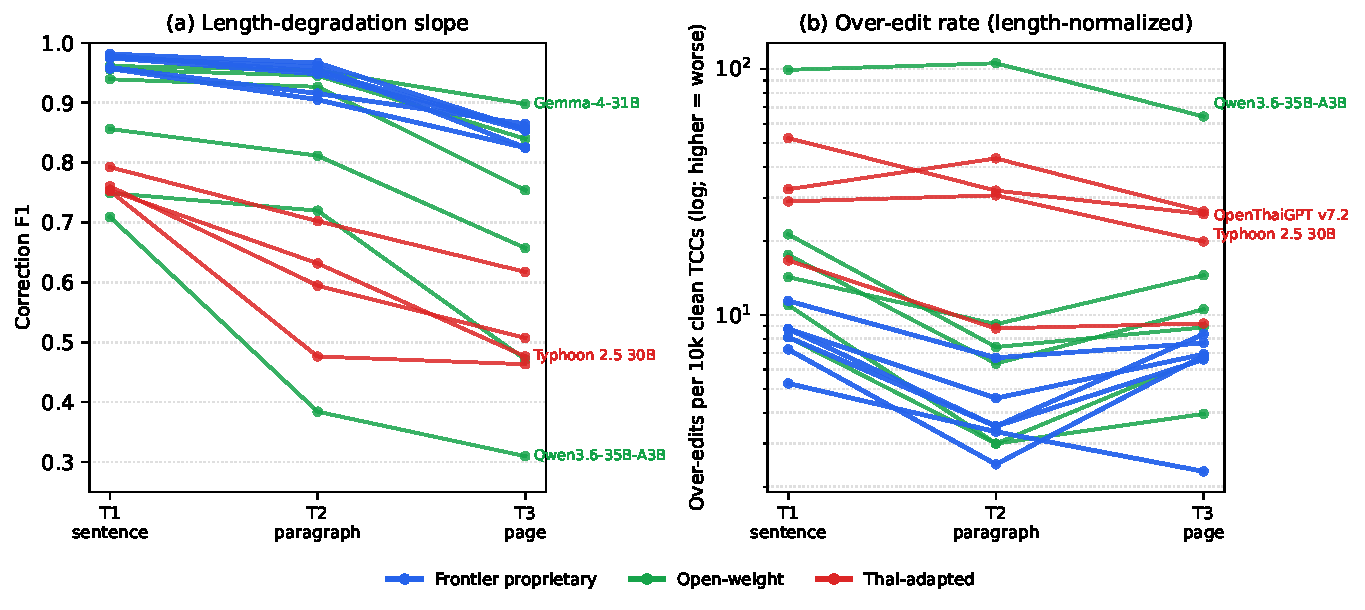
\includegraphics[width=\textwidth]{fig1-degradation.pdf}
\caption{Length robustness. \emph{(a)}~Correction-F1 slope from T1 to T3. The frontier (blue)
and the strongest open-weight model (Gemma-4, green) stay high while weak models slope off.
\emph{(b)}~Over-edit rate per 10{,}000 clean TCCs on a log scale, where higher is worse. The
rate is roughly flat across length, so the per-passage accumulation (the absolute counts in this appendix)
reflects text exposure rather than a rising false-positive rate. Weak models over-edit at many
times the frontier's per-unit rate at every tier.}
\label{fig:degradation}
\end{figure*}

\begin{table*}[t]
\centering\small\setlength{\tabcolsep}{8pt}
\begin{tabular}{@{}lccc@{}}
\toprule
model & T1 & T2 & T3 \\
\midrule
GPT-5.5 (high)            & [0.964, 0.980] & [0.952, 0.984] & [0.803, 0.902] \\
GPT-5.5 (med)             & [0.960, 0.977] & [0.934, 0.974] & [0.806, 0.902] \\
Claude Opus 4.7           & [0.958, 0.978] & [0.924, 0.970] & [0.778, 0.911] \\
Gemini 3.5 Flash          & [0.955, 0.975] & [0.942, 0.976] & [0.759, 0.874] \\
Gemma-4-31B               & [0.938, 0.962] & [0.931, 0.974] & [0.846, 0.928] \\
GPT-5.4-mini              & [0.936, 0.960] & [0.888, 0.944] & [0.810, 0.893] \\
Claude Sonnet 4.6         & [0.933, 0.959] & [0.875, 0.936] & [0.753, 0.890] \\
DeepSeek V4 Flash         & [0.935, 0.959] & [0.918, 0.968] & [0.775, 0.880] \\
DeepSeek V4 Pro           & [0.912, 0.939] & [0.902, 0.949] & [0.684, 0.806] \\
GLM-5.1                   & [0.823, 0.867] & [0.767, 0.855] & [0.545, 0.781] \\
Typhoon-S 8B$^\dagger$    & [0.759, 0.805] & [0.652, 0.751] & [0.552, 0.683] \\
THaLLE 8B$^\dagger$       & [0.715, 0.780] & [0.540, 0.649] & [0.436, 0.598] \\
Typhoon 2.5 30B$^\dagger$ & [0.716, 0.767] & [0.580, 0.684] & [0.399, 0.538] \\
OpenThaiGPT v7.2$^\dagger$& [0.701, 0.777] & [0.386, 0.571] & [0.380, 0.534] \\
MiniMax-M2.7              & [0.714, 0.765] & [0.671, 0.767] & [0.392, 0.552] \\
Qwen3.6-35B-A3B           & [0.673, 0.736] & [0.308, 0.470] & [0.227, 0.419] \\
\bottomrule
\end{tabular}
\caption{95\% item-bootstrap confidence intervals on correction F1 (10{,}000
resamples). $\dagger$ $=$ Thai-native.}
\label{tab:ci}
\end{table*}

\begin{table}[t]
\centering\small\setlength{\tabcolsep}{4pt}
\begin{tabular}{@{}lccc@{}}
\toprule
class & T1 & T2 & T3 \\
\midrule
1 tone mark          & 0.896 & 0.868 & 0.807 \\
2 consonant-pair     & 0.876 & 0.885 & 0.831 \\
3 silent-consonant   & 0.887 & 0.865 & 0.800 \\
4 vowel              & 0.857 & 0.870 & 0.854 \\
5 cluster/metathesis & 0.863 & 0.807 & 0.838 \\
6 loanword           & 0.808 & 0.802 & 0.819 \\
\midrule
all classes          & 0.866 & 0.851 & 0.828 \\
spread (max$-$min)   & 0.088 & 0.083 & 0.054 \\
\bottomrule
\end{tabular}
\caption{Fraction of gold edits fixed, by mechanism class and tier, pooled over all 16 models.
Gold-edit counts per cell are in Table~\ref{tab:classcounts}.}
\label{tab:mech}
\end{table}

\textbf{Pooled per-class outcome split (T1, all 16 models).}
\begin{center}\small\setlength{\tabcolsep}{3pt}
\begin{tabular}{@{}lrrrr@{}}
\toprule
class & gold edits & fixed & miscorrected & missed \\
\midrule
1 tone     & 2{,}608 & 0.896 & 0.011 & 0.092 \\
2 consonant& 2{,}192 & 0.876 & 0.006 & 0.117 \\
3 silent-consonant & 2{,}640 & 0.887 & 0.010 & 0.103 \\
4 vowel    & 2{,}896 & 0.857 & 0.002 & 0.140 \\
5 cluster  & 3{,}392 & 0.863 & 0.012 & 0.126 \\
6 loanword & 1{,}968 & 0.808 & 0.003 & 0.189 \\
\bottomrule
\end{tabular}
\end{center}
\textbf{Over-edits per 100 items across tiers (absolute accumulation).}
\begin{center}\small
\begin{tabular}{@{}lrrr@{}}
\toprule
model & T1 & T2 & T3 \\
\midrule
GPT-5.5 (med)    & 7  & 8   & 41  \\
Gemma-4-31B      & 6  & 8   & 32  \\
GLM-5.1          & 10 & 23  & 106 \\
Typhoon 2.5 30B  & 32 & 82  & 201 \\
OpenThaiGPT v7.2   & 20 & 110 & 206 \\
Qwen3.6-35B-A3B  & 59 & 268 & 484 \\
\bottomrule
\end{tabular}
\end{center}
\textbf{Over-edit rate per 10{,}000 clean TCCs (length-normalized; the
Figure~\ref{fig:degradation}b data).} The per-unit rate is roughly flat or falls across tiers,
so the per-item growth above reflects text exposure, not a rising false-positive rate.
\begin{center}\small
\begin{tabular}{@{}lrrr@{}}
\toprule
model & T1 & T2 & T3 \\
\midrule
GPT-5.5 (med)    & 12.3  & 3.0   & 5.5  \\
Gemma-4-31B      & 11.4  & 3.0   & 4.3  \\
GLM-5.1          & 17.8  & 9.3   & 14.3 \\
Typhoon 2.5 30B  & 56.8  & 32.6  & 27.0 \\
OpenThaiGPT v7.2   & 35.0  & 44.0  & 27.8 \\
Qwen3.6-35B-A3B  & 105.4 & 106.8 & 65.1 \\
\bottomrule
\end{tabular}
\end{center}
\textbf{Register effect (pooled correction recall, T1/T2/T3).} encyclopedic 0.82/0.79/0.71;
news 0.87/0.85/0.76; government 0.89/0.90/0.83. Per-model $\times$ class correction recall and
span-F0.5 per type are released with the data.

\section{Annotation study}
\label{app:annotation}
\textbf{Design.} The 60 items comprise the 40 curated mined items (Appendix~\ref{app:construction})
and 20 synthetic items chosen
so that each automatic class has ten items. Each item shows one marked span with its proposed
correction. Raters answer two questions per item: whether the marked span is a genuine
orthographic error, and which of the six classes it belongs to, following a written guideline
with the class definitions and the two conventions of Appendix~\ref{app:taxonomy}. No automatic
label is shown. The two raters, one of them an author, worked independently. Etymology and edit-operation tags are not
annotated, since they are a dictionary lookup and a deterministic function of the edit.

\textbf{Results.} Error validity: both raters accepted all 60 spans. Class agreement:
Krippendorff's $\alpha = 0.752$ (nominal, $n = 60$). Table~\ref{tab:alpha} gives one-vs-rest
$\alpha$ and raw agreement per automatic class; with ten items per class these values are noisy.

\begin{table}[t]
\centering\small\setlength{\tabcolsep}{4pt}
\begin{tabular}{@{}lcc@{}}
\toprule
automatic class & $\alpha$ (one-vs-rest) & agreement \\
\midrule
1 tone mark          & 0.793 & 1.00 \\
2 consonant-pair     & 0.921 & 0.90 \\
3 silent-consonant   & 0.611 & 0.60 \\
4 vowel              & 0.773 & 0.70 \\
5 cluster/metathesis & 1.000 & 1.00 \\
6 loanword           & 0.485 & 0.60 \\
\midrule
all (multiclass)     & 0.752 & 0.80 \\
\bottomrule
\end{tabular}
\caption{Inter-rater agreement per automatic class (ten items each).}
\label{tab:alpha}
\end{table}

\textbf{Where labels differ.} The raters split on 12 items and agree with each other against the
automatic label on 13. Of these 25, 17 involve the loanword-absorption rule in one of two
directions: raters labeled the surface mechanism of a contemporary loan (for example, a
consonant swap in เวียตนาม$\to$เวียดนาม rated class~2 rather than 6), or recognized a loan that
the loan lexicon missed (เยอรมันนี$\to$เยอรมนี, typed class~5 but rated 6); old borrowings such
as เวทมนตร์ split the raters between class~3 and~6. Four more are homophone swaps outside the
Indic-origin groups (ฅน$\to$คน three times, and กบถ$\to$กบฏ), which the taxonomy places in
class~5 and both raters placed in class~2. The remaining four concern whether a stray or
misplaced diacritic counts as a tone-mark, vowel, or silent-consonant error. The disagreements
therefore sit at the class boundaries fixed by convention rather than at error perception.

\section{Natural-error evaluation}
\label{app:natural}
The natural set comes from the edit history of a Thai Wikipedia spelling-cleanup bot: 103 items, each a
real error in its original encyclopedic sentence, with the bot's fix as gold. We apply the consensus
audit of Section~\ref{sec:qc} with the same threshold ($k = 3$). It drops an item when the consensus
output makes a spelling change the gold does not, and keeps it when the consensus equals the input,
differs only in whitespace or punctuation, or is a partial fix on the way to the gold. It removes
24 items: in 20 the consensus also fixes a second, unmarked error elsewhere in the sentence
(for example เพึย$\to$เพีย), and in 4 the recorded fix is itself incomplete (ตำ่ recorded as ตำ, น้้า as น้า, and
สรา้ง as สราง, where the intended words are ต่ำ, น้ำ, and สร้าง). The audited set has 79 items and 80 gold
edits (automatic classes 1: 24, 2: 19, 3: 13, 4: 18, 5: 5). Table~\ref{tab:natural} gives per-model results on
the audited set, with correction F1 and the miscorrected share on all 103 items for comparison. On the audited set the ranking correlates
with the T1 ranking at Spearman $\rho = 0.92$ (Pearson $r = 0.93$); on all 103 items, at $\rho = 0.88$ ($r = 0.93$).

\begin{table*}[t]
\centering\small
\begin{tabular}{@{}lcccccccc@{}}
\toprule
 & \multicolumn{6}{c}{audited set ($n = 79$)} & \multicolumn{2}{c}{all items ($n = 103$)} \\
\cmidrule(lr){2-7}\cmidrule(l){8-9}
model & corr F1 & 95\% CI & det F1 & fixed & miscorrected & missed & corr F1 & miscorrected \\
\midrule
GPT-5.5 (high)              & \textbf{0.943} & [0.907, 0.975] & 0.943 & 0.938 & 0.000 & 0.062 & 0.800 & 0.048 \\
Gemma-4-31B                 & \tie{0.942} & [0.893, 0.981] & 0.955 & 0.912 & 0.013 & 0.075 & 0.819 & 0.058 \\
GPT-5.5 (med)               & \tie{0.931} & [0.886, 0.969] & 0.931 & 0.925 & 0.000 & 0.075 & 0.791 & 0.048 \\
GPT-5.4-mini                & \tie{0.917} & [0.859, 0.969] & 0.930 & 0.900 & 0.013 & 0.087 & 0.811 & 0.058 \\
Claude Opus 4.7             & \tie{0.892} & [0.785, 0.968] & 0.892 & 0.925 & 0.000 & 0.075 & 0.791 & 0.038 \\
Claude Sonnet 4.6           & 0.882 & [0.810, 0.942] & 0.895 & 0.838 & 0.013 & 0.150 & 0.771 & 0.058 \\
Gemini 3.5 Flash            & \tie{0.865} & [0.750, 0.969] & 0.865 & 0.963 & 0.000 & 0.037 & 0.757 & 0.038 \\
DeepSeek V4 Flash           & 0.841 & [0.750, 0.921] & 0.841 & 0.825 & 0.000 & 0.175 & 0.757 & 0.048 \\
DeepSeek V4 Pro             & 0.818 & [0.727, 0.909] & 0.818 & 0.900 & 0.000 & 0.100 & 0.729 & 0.038 \\
GLM-5.1                     & 0.759 & [0.663, 0.853] & 0.759 & 0.750 & 0.000 & 0.250 & 0.689 & 0.048 \\
Typhoon 2.5 30B$^\dagger$   & 0.740 & [0.649, 0.831] & 0.751 & 0.800 & 0.013 & 0.188 & 0.655 & 0.048 \\
THaLLE 8B$^\dagger$         & 0.727 & [0.638, 0.811] & 0.727 & 0.650 & 0.000 & 0.350 & 0.670 & 0.048 \\
OpenThaiGPT v7.2$^\dagger$    & 0.717 & [0.623, 0.806] & 0.717 & 0.650 & 0.000 & 0.350 & 0.630 & 0.048 \\
MiniMax-M2.7                & 0.702 & [0.607, 0.785] & 0.702 & 0.588 & 0.000 & 0.412 & 0.663 & 0.038 \\
Typhoon-S 8B$^\dagger$      & 0.687 & [0.587, 0.774] & 0.702 & 0.562 & 0.013 & 0.425 & 0.626 & 0.038 \\
Qwen3.6-35B-A3B             & 0.567 & [0.468, 0.670] & 0.606 & 0.738 & 0.050 & 0.212 & 0.544 & 0.067 \\
\bottomrule
\end{tabular}
\caption{Natural-error evaluation. \textbf{Bold} $=$ best on the audited set; \underline{underlined}
$=$ not separable from the best by a paired bootstrap test ($p \ge 0.05$); $\dagger$ $=$ Thai-native.}
\label{tab:natural}
\end{table*}

\section{Prompt and inference}
\label{app:prompt}
A single fixed Thai instruction prompt is used for all models. It asks the model to return the
passage with orthographic errors corrected and \textbf{nothing else changed}, explicitly
forbidding spacing, punctuation, and numeral edits. Temperature is 0 where supported. Claude
models use the Anthropic Message Batches API in non-thinking mode. GPT-5.x models use the
Responses API at the stated reasoning effort with a 3k-token budget. Open reasoning models run
in native thinking mode with large token budgets, and token-runout counts as a failure.
ThaiLLM-gateway models are reached with a browser User-Agent header, because the gateway's
web application firewall otherwise blocks the default SDK user agent.

\textbf{Prompt sensitivity.} We rerun the full T1 set for one strong general model (Gemma-4-31B)
and one Thai 8B model (Typhoon-S) under two alternative prompts: the same instruction in English,
and the Thai instruction with two worked examples from the train split, which is disjoint from T1 (Table~\ref{tab:prompt}).
Prompt choice shifts correction F1 by at most 0.07, and Gemma-4 stays ahead of Typhoon-S under
every prompt. The two models move in opposite directions: the worked examples help the Thai 8B
model and hurt the general model.

\begin{table}[t]
\centering\small\setlength{\tabcolsep}{4pt}
\begin{tabular}{@{}lccc@{}}
\toprule
model & Thai (default) & English & Thai + 2 examples \\
\midrule
Gemma-4-31B & 0.950 & 0.924 & 0.885 \\
Typhoon-S 8B & 0.782 & 0.799 & 0.834 \\
\bottomrule
\end{tabular}
\caption{T1 correction F1 under three prompts ($n = 795$).}
\label{tab:prompt}
\end{table}

\end{document}
